\vspace{3mm}
\subsection{Traffic Volume- Voice}

users can filter and view the traffic volume for **Voice** data over the selected period. The available filters include **Traffic Type**, **Period**, **Operators**, **Network Category**, **Direction**, and **Start/End Date**. Users can also apply **Quick Presets** such as **Last Hour**, **24 Hours**, or **7 Days** to quickly adjust the view based on their needs.

Once the filters are applied, the results are displayed in both graphical and tabular formats. This helps users quickly analyze the traffic patterns for the selected period and operator.

\begin{figure}[H]
  \centering
  \colorbox{gray!20}{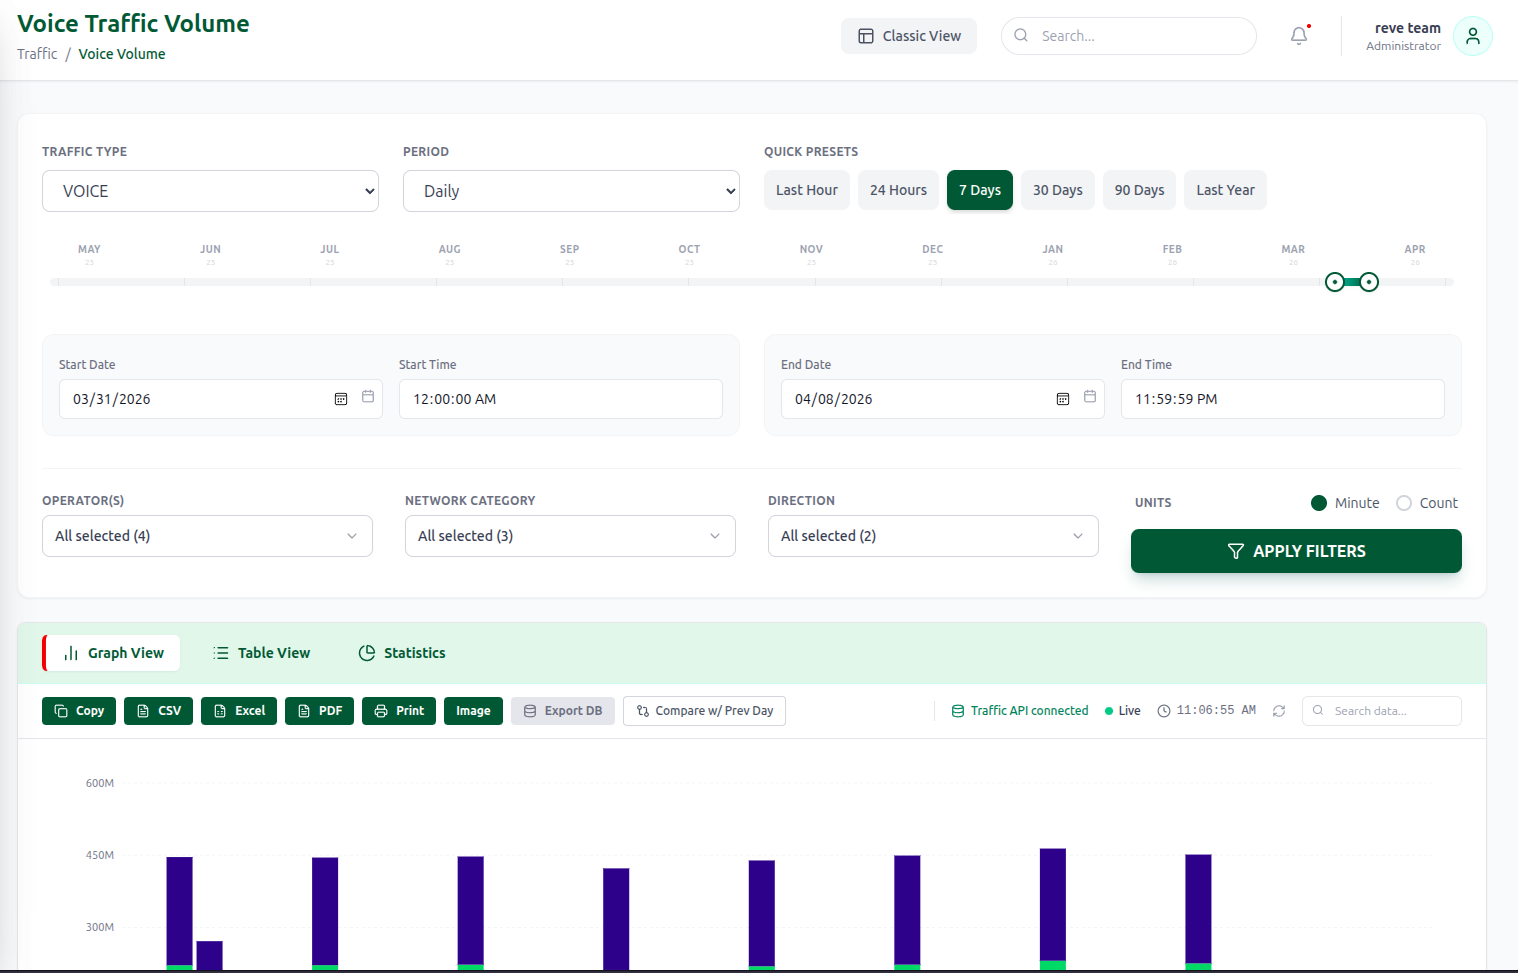
\includegraphics[width=.97\textwidth]{img/traffic/voice/Traficvoicepageview.png}}  % Replace with the path to your image file
  \caption{Example of Voice Traffic Volume Dashboard}
\end{figure}
% -------------------------------------Traffic Volume - Voice Search Filters-------------------------------------

\subsubsection{Traffic Volume- Voice Search Filters}
In this section, users can filter traffic volume data
by selecting the appropriate parameters for Voice traffic.
To perform a voice search, the user needs to select the **Voice** option in the traffic type filter.
This will allow the user to view only the voice traffic data\\
\vspace{3mm}
\textbf{Traffic Type:} For Voice traffic, the user can select from the following options:

\begin{figure}[ht]

  \begin{minipage}[b]{0.20\textwidth}
    \begin{itemize}
      \item Voice
      \item \st{SMS}
      \item \st{Data}
      \item \st{ICX In/Out}
      \item \st{IGW In/Out}
    \end{itemize}
  \end{minipage}
  \hfill
  \begin{minipage}[t]{0.35\textwidth}
    \centering
    \colorbox{gray!20}{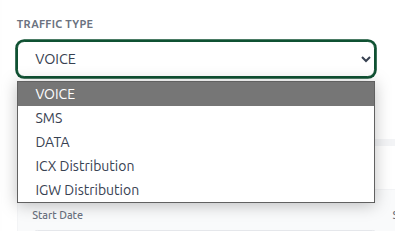
\includegraphics[width=0.95\textwidth]{img/traffic/trafficTypes.png}}
    \caption{Traffic Type Selection}
  \end{minipage}

\end{figure}
\vspace{3mm} %3mm vertical space
\textbf{Period:} The user can select a time period for data view, which can be one of the following:
\vspace{-10pt}
\begin{figure}[h]
  \begin{minipage}[b]{0.40\textwidth}

    \begin{itemize}
      \item Hourly
      \item Daily
      \item Monthly
      \item Yearly
    \end{itemize}
  \end{minipage}
  \hfill
  \begin{minipage}[t]{0.35\textwidth}
    \centering
    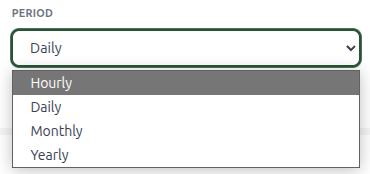
\includegraphics[width=\textwidth]{img/common/commonarea/period.png}  % Replace with the path to your image file
    \caption{Example of Period Selection}
  \end{minipage}
\end{figure}\\
\vfill
\vspace{3mm} %3mm vertical space
\textbf{Quick Presets:} The user can quickly select a preset time range from the following options:

\begin{figure}[h]

  \begin{minipage}[]{0.40\textwidth}
    \begin{itemize}
      \item Last Hour
      \item Last 24 Hours
      \item Last 7 Days
      \item Last 30 Days
      \item Last 90 Days
      \item Last Year
    \end{itemize}
  \end{minipage}
  \begin{minipage}[t]{0.45\textwidth}
    \centering
    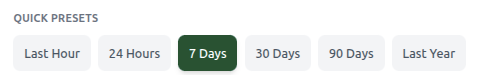
\includegraphics[width=\textwidth]{img/common/commonarea/QuickPresents.png}  % Replace with the path to your image file
    \caption{Example of Quick Preset Selection}
  \end{minipage}

\end{figure}
\vfill

\vspace{3mm} %3mm vertical space
\textbf{Start \& End Date and Time:} The user selects the start date and, if the "Hourly" period is selected, the start time. The end date and end time are also configurable, but the start and end time are only active for the "Hourly" period.\\
\begin{figure}[htbp]
  \centering
  \begin{subfigure}[b]{0.40\textwidth}
    \centering
    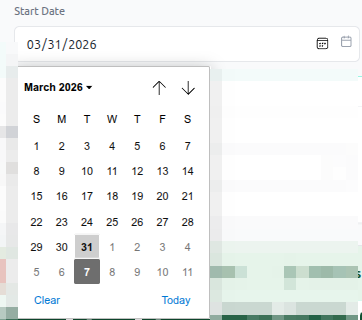
\includegraphics[width=\linewidth,valign=b]{img/common/commonarea/StartDate.png}
    \caption{Start \& End Date Selection}
    \label{fig:img1}
  \end{subfigure}
  \hfill
  \begin{subfigure}[b]{0.40\textwidth}
    \centering
    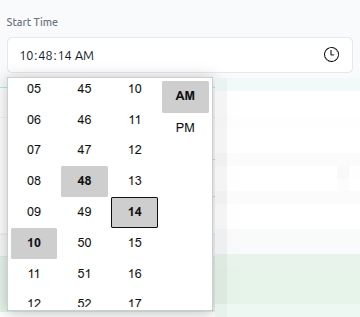
\includegraphics[width=\linewidth,valign=b]{img/common/commonarea/StartTime.png}
    \caption{Start \& End Time Selection}
    \label{fig:img2}
  \end{subfigure}
  \caption{Overall figure caption (optional).}
  \label{fig:side_by_side}
\end{figure}
\vfill
\textbf{Quick Time Selection}

In this section, users can quickly set the desired time range for their data analysis. By using the time selection slider, users can adjust the range by simply moving the indicator along the timeline. This allows for a smooth and intuitive way to select specific periods for viewing data. The slider lets users choose from various predefined time frames, such as Last Hour, Last 24 Hours, and more.

\begin{figure}[h]
  \centering
  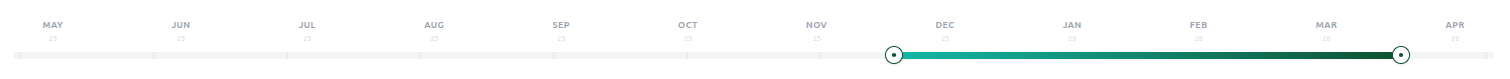
\includegraphics[width=\textwidth]{img/common/commonarea/QuickTimeSelection.png}
  \caption{Example of Quick Time Selection}
\end{figure}

As the user moves the slider, the time range is automatically updated, reflecting the selected period. This feature provides a dynamic and user-friendly interface for analyzing data across different time intervals.

\vspace{5mm} %3mm vertical space
\textbf{Operators:} The user can select operators as needed. The options include:
\begin{itemize}
  \item All operators
  \item Single operator
  \item Multiple operators
\end{itemize}

\vspace{3mm}
\textbf{Network Category:} The user can choose from various network categories, with all categories being selected by default.\linebreak
\begin{figure}[ht]
  \centering
  \itshape
  \colorbox{gray!20}{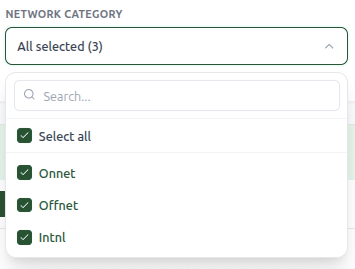
\includegraphics[width=0.35\textwidth]{img/traffic/NetworkCatagory.png}}
  \caption{Example of Network Category Selection}
\end{figure}
\clearpage

\vspace{3mm}
\textbf{Direction:} The user can choose the direction for the traffic (Incoming or Outgoing), with all directions being selected by default.\\
\begin{figure}[ht]
  \centering
  \itshape
  \colorbox{gray!20}{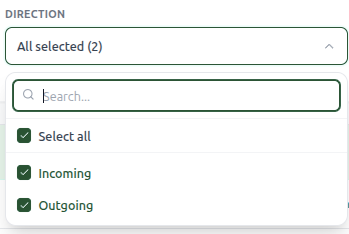
\includegraphics[width=0.30\textwidth]{img/traffic/trafficDirection.png}}
  \caption{Example of Traffic Direction Selection}
\end{figure}
\vspace{3mm}
%\textbf{Units:} The user can select between two unit types:
\includegraphics[width=0.3\textwidth]{img/traffic/minuteCount.png}\\
\textbf{Units:} The user can select between two unit types: \raisebox{-0.2\height}{
\includegraphics[height=2em]{img/traffic/minuteCount.png}}
\begin{itemize}
  \item Minute
  \item Count
\end{itemize}

After \textbf{APPLY FILTERS},\colorbox{gray!20}{
\includegraphics[width=0.2\textwidth]{img/common/commonarea/Applyfilter.png}} the search results will update to reflect the selected parameters.

\par\vspace{5mm}

% -----------------------------Traffic Volume - Voice Search Results-------------------------------------

\subsubsection{Traffic Volume - Voice Search Results}

In this section, users can view the results for the **Voice Traffic** based on the filters applied. The data is displayed in a table format, showing detailed information for each operator and period. Users can view and analyze the traffic metrics such as inbound and outbound traffic, international traffic, and total minutes for the selected period.

The table also allows users to perform actions like downloading the results in different formats (CSV, Excel, PDF), copying, or printing the data. Additionally, users can compare the data with the previous day's traffic using the "Compare w/ Prev Day" option.

\begin{figure}[h]
  \centering
  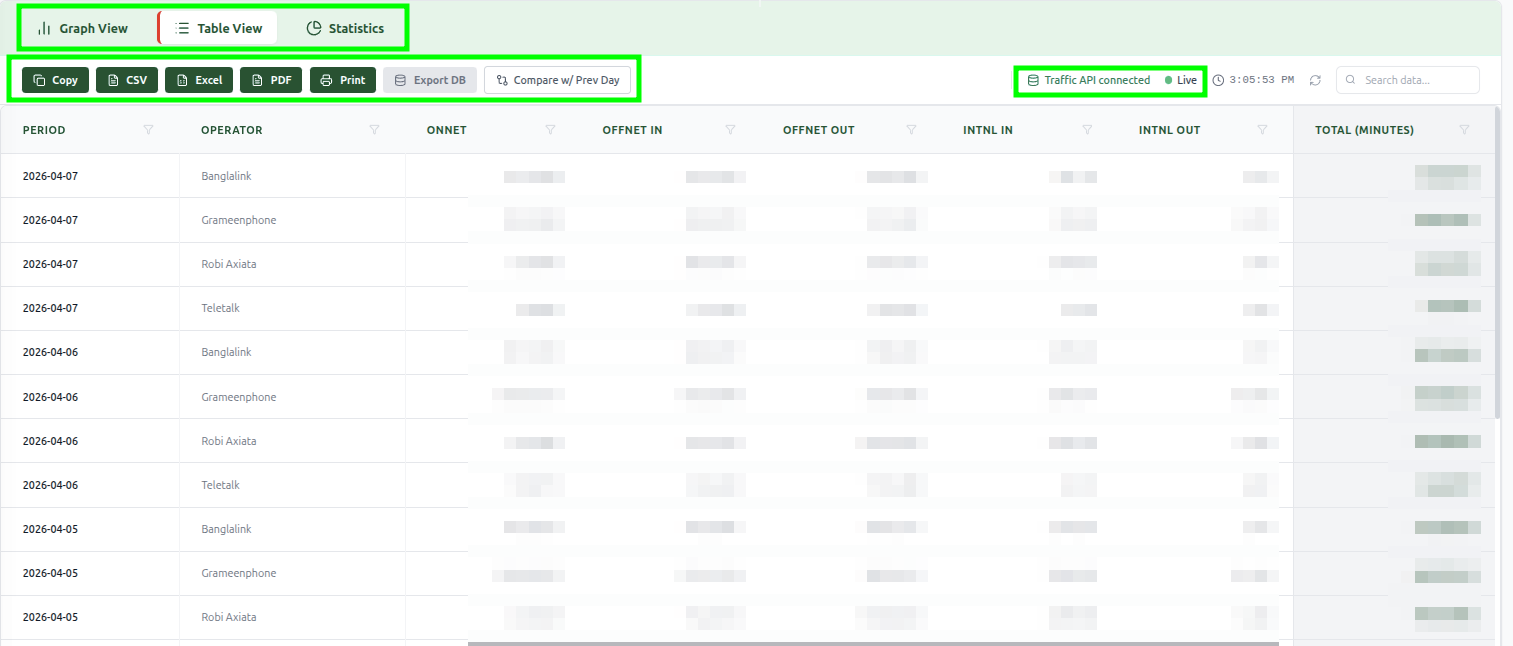
\includegraphics[width=\textwidth]{img/traffic/voice/VoiceTableView.png}  % Replace with the path to your image file
  \caption{Example of Voice Search Results Table View}
\end{figure}
\clearpage
\par\vspace{3mm}
{\large \textbf{Custom Search Results Header:}}

In this section, users can interact with various features for downloading, viewing, and interacting with the results:
\begin{figure}[H]
  \centering  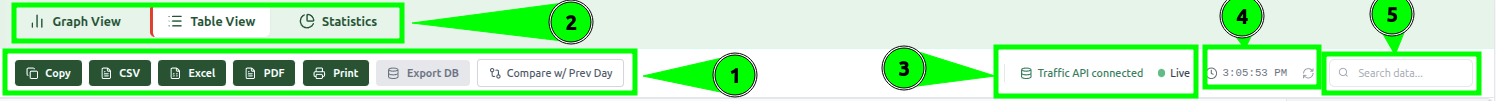
\includegraphics[width=\textwidth]{img/common/commonarea/results/ResultsCommonArea.png}

  \caption{Example of Results Common Area}
\end{figure}
\begin{enumerate}
  \item \textbf{Download and Export Options:}
    Users can download the custom results in different formats such as \textbf{CSV}, \textbf{Excel}, \textbf{PDF}, or \textbf{Copy}, or they can choose to print the results. Additionally, users can export the data directly from the database and compare it with the previous day's data.

  \item \textbf{View Options:}
    Users can view the results in different modes:
    \begin{itemize}
      \item Graph View – Display the results in a graphical format.
      \item Table View – View the results in a tabular format.
      \item Statistics – View the detailed statistics.
    \end{itemize}

  \item \textbf{Traffic API Status:}
    It is crucial to check whether the \textbf{Traffic API} is connected. If the API is disconnected, data may not load, and the user might not be able to view the required results.

  \item \textbf{Server Time:}
    The \textbf{Server Time} is displayed to indicate the current time of the server, which can be useful for comparing time-sensitive data.

  \item \textbf{Search Area:}
    The user can utilize the \textbf{Search Area} to search for specific data within the results table.
\end{enumerate}

{
  \par\vspace{5mm}
  {\large \textbf{Table Sorting and Filtering}}
  \par\vspace{3mm}

  In this section, users can sort and filter the data to view the results based on specific criteria.
  \par\vspace{3mm}
  \textbf{1. Sorting:}
  Users can click on the **column headers** to sort the data in ascending or descending order. This allows for a better-organized view of the data according to the selected column.
  \par\vspace{2mm}
  \textbf{2. Filtering}:
  Users can apply custom filters to the displayed results by using the filter icon. By clicking on the **filter icon** (highlighted in the image), a dropdown menu appears where users can search for specific values and select which options they want to filter by. This feature allows users to focus on the data they are interested in, such as selecting specific operators (e.g., **Banglalink**, **Grameenphone**, **Teletalk**).

  \begin{figure}[H]
    \centering
    \colorbox{gray!20}{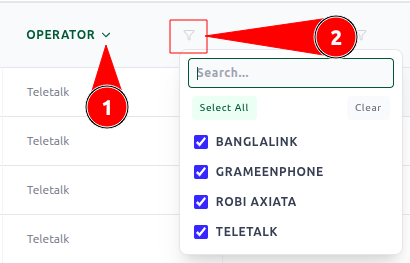
\includegraphics[width=.25\textwidth]{img/common/commonarea/results/R4TableSortingFilter.png}}  % Replace with the path to your image file
    \caption{Example of Table Sorting and Filtering}
  \end{figure}
}
\par\vspace{5mm}
{\large \textbf{Traffic Volume - Compare with Previous Day}}

When the user selects the **"Compare w/ Prev Day"**\colorbox{gray!20}{
\includegraphics[width=0.2\textwidth]{img/common/commonarea/results/CompareTheDaySmall.png}} option, the data displayed will include a comparison with the previous day's traffic data. This feature allows users to easily view how traffic has changed from one day to the next. The comparison is shown in terms of both the traffic volume and the percentage change.

As shown in the example below, users can see the differences in the traffic data for each operator. The data is displayed alongside arrows indicating whether the traffic has increased or decreased, along with the percentage change from the previous day.

\begin{figure}[ht]
  \centering
  \colorbox{gray!20}{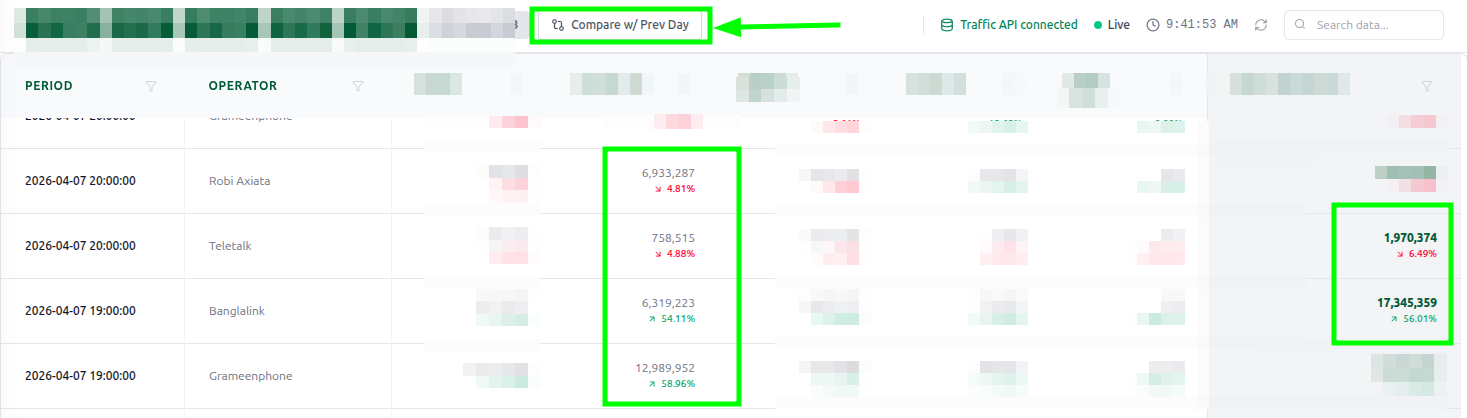
\includegraphics[width=.97\textwidth]{img/common/commonarea/results/CompareTheDay.png}}  % Replace with the path to your image file
  \caption{Example of Traffic Volume Comparison with Previous Day}
\end{figure}

This feature helps users quickly assess performance and identify trends in traffic over time.

\par\vspace{5mm}
{\large \textbf{Pagination}}
\par\vspace{3mm}
In this section, users can view the results in a paginated format. The pagination control allows users to select the number of rows they want to display per page. Options such as **20**, **50**, **100**, and **200** rows can be selected, providing flexibility in viewing the data.

On the right side, there are navigation arrows that allow the user to move between pages. The **Previous** and **Next** buttons help users navigate through the results, while the current page number is displayed for clarity. This allows for easy browsing of large datasets without overwhelming the user with too much information at once.

\begin{figure}[ht]
  \centering  \colorbox{gray!20}{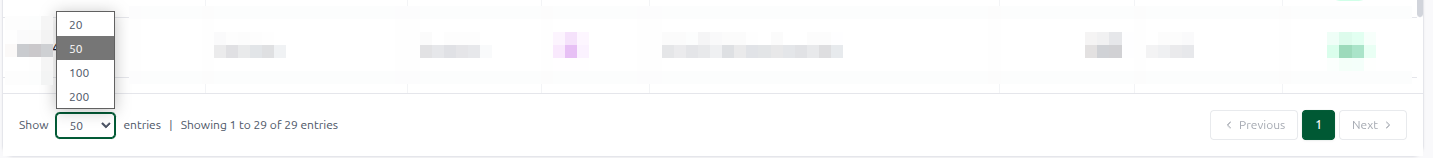
\includegraphics[width=.97\textwidth]{img/common/commonarea/results/R3Pageination.png}}  % Replace with the path to your image file

  \caption{Example of Pagination Control}
\end{figure}